\chapter{Wechselwirkung von Elektronen und Photonen mit Materie}
\section{Elektronen}
\begin{figure}
	\centering
	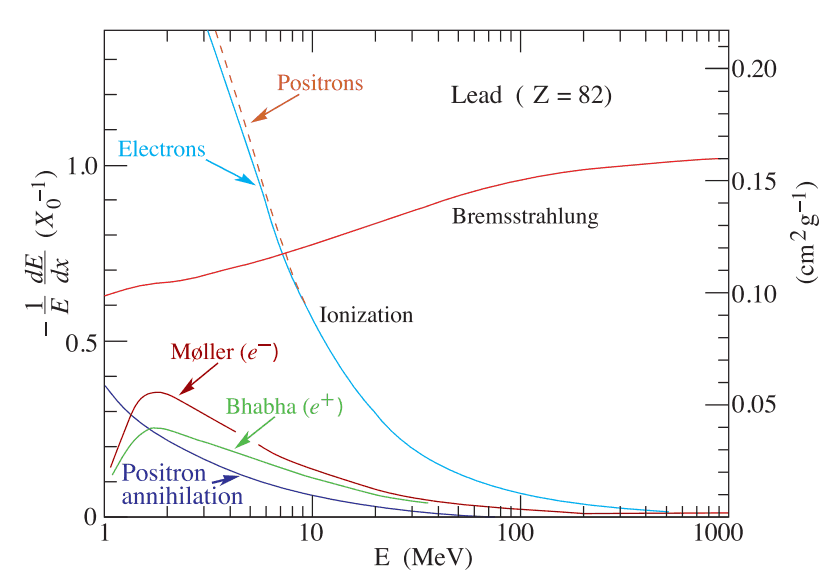
\includegraphics[width=.7\textwidth]{./img/electroninteractions.jpg}
	\caption{Energieverlust vs. Energie von verschiedenen Prozessen}
	\label{fig:electroninteractions}
\end{figure}
Elektronen können, je nach ihrer Energie, auf verschiedene Weisen mit Materie wechselwirken.
Dazu gehören die Prozesse
\begin{itemize}
	\item Möller-Streuung (einfach nur e an e)
	\item Bhabha-Streuung (einfach nur e an pos)
	\item Paarvernichtung und
	\item Bremsstrahlung
	\item Cherenkovstrahlung.
\end{itemize}
\autoref{fig:electroninteractions} zeigt den Energieverlust für verschiedene Energien und Prozesse.
Bremsstrahlung ist für hohe Energien dominant, Streuung und Ionisation für niedrige Energien.
Die \textbf{kritische Energie} ist dabei der Punkt, ab dem die Verluste durch Ionisation und Strahlung gleich sind.
Die Strahlungslänge $X_0$ ist definiert über
\begin{equation*}
	-\diff[E]{X} = \frac{E}{X_0}.
\end{equation*}

\subsection{Energieverlust durch Ionisation}
Die wichtigste Wechselwirkung geladener Teilchen ist die Ionisation des aktiven Mediums.
Dabei führt das Teilchen elastische Stöße mit den gebundenen Elektronen in den Atomen des Mediums aus.
Dies führt zu einem charakteristischen Energieverlust nach der \textbf{Bethe-Formel}
\begin{equation*}
	\diff[E]{X}\propto -z^2n_e\cdot\frac{1}{\beta^2}\log\left(\frac{2m_e\beta^2\gamma^2}{I} - \beta^2\right)
\end{equation*}
mit der Ladungszahl des Teilchens $z$, der Elektronendichte $n_e$ und der Ionisationsenergie $I$, welche mediumspezifisch ist.

Es fällt auf, dass die Ionisationsverluste unabhängig von der Masse des Teilchens sind.

Die Bethe-Formel beschreibt allerdings nur den mittleren Energieverlust.
Insbesondere in dünnen Absorbern führt dies zu von Fall zu Fall asymmetrischen Verteilungen.
Diese Fluktuationen werden empirisch durch die \textbf{Landau-Verteilung} beschrieben.

\subsection{Energieverlust durch Bremsstrahlung}
\begin{figure}
	\centering
	\begin{subfigure}{0.4\textwidth}
		\centering
		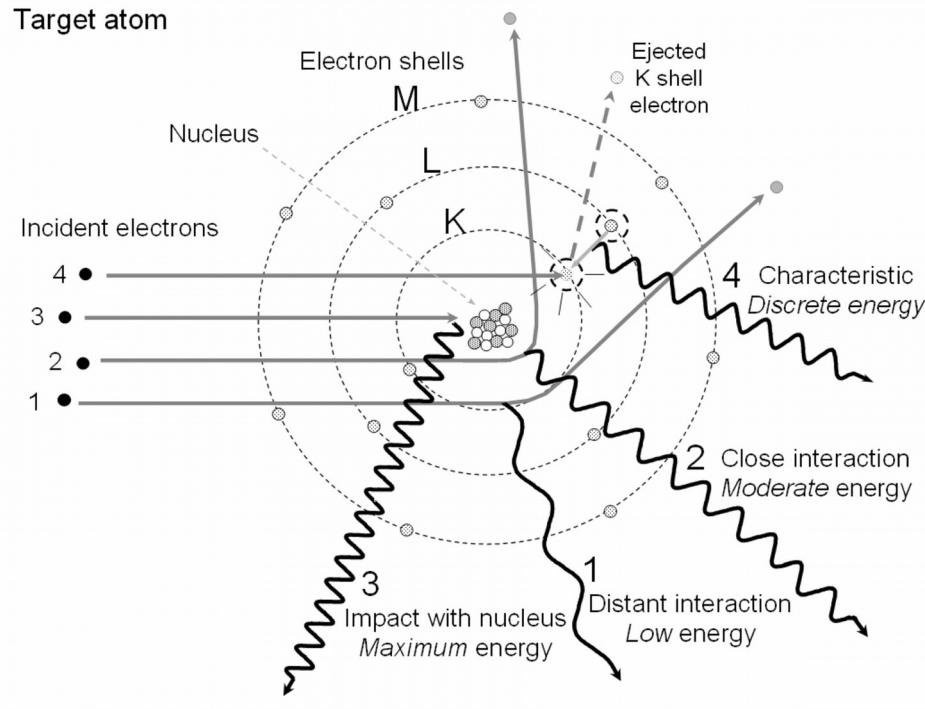
\includegraphics[width=\textwidth]{./img/elatom.jpg}
		\caption{Der Prozess der Bremsstrahlung}
		\label{fig:elatom}
	\end{subfigure}
	\begin{subfigure}{0.4\textwidth}
		\centering
		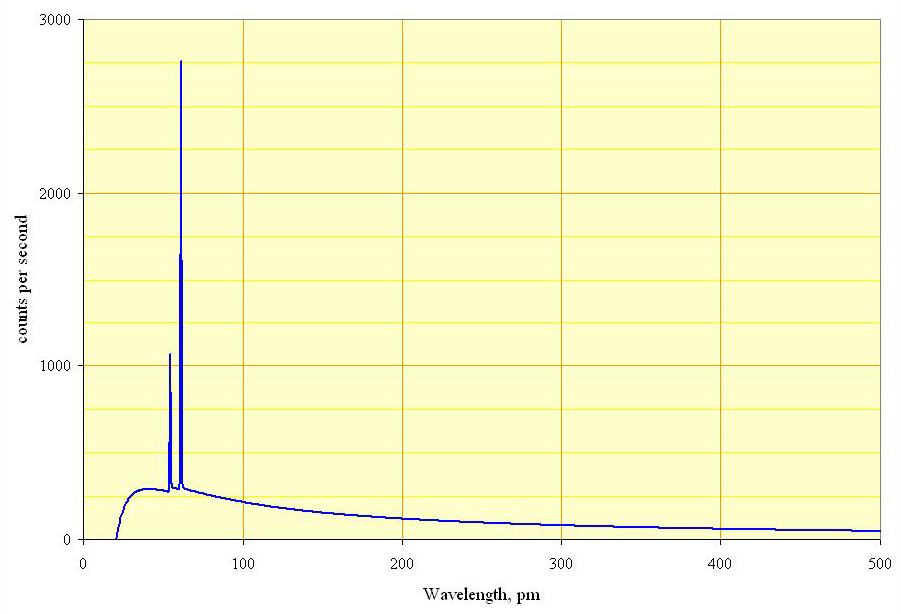
\includegraphics[width=\textwidth]{./img/bremsspec.jpg}
		\caption{Bremsstrahlungsspektrum mit überlagerten Floureszenzpeaks}
		\label{fig:bremsspec}
	\end{subfigure}
\end{figure}
Wird ein geladenes Teilchen beschleunigt, so emittiert es Bremsstrahlung.
Dabei ist die totale Strahlungsleistung für eine geradlinige Bewegung und eine Beschleunigung parallel zur Geschwindigkeit
\begin{equation*}
	P_\parallel = \frac{q^2a^2\gamma^6}{6\pi\varepsilon_0c^3}.
\end{equation*}
Wird das Teilchen allerdings orthogonal zu seiner Bewegungsrichtung beschleunigt (Kreisbahn), so ist
\begin{equation*}
	P_\perp = \frac{q^2a^2\gamma^4}{6\pi\varepsilon_0c^3}.
\end{equation*}
Da $\gamma = \frac{E}{mc^2}$ ist der Verlust durch Bremsstrahlung für schwere Teilchen deutlich geringer als für leichte.
Daher kann ein Elektronbeschleuniger im \si{\TeV}-Bereich aufgrund der geringen Elektronmasse niemals als Ringbeschleuniger realisiert werden, sondern nur als Linearbeschleuniger.

\autoref{fig:elatom} veranschaulicht den Prozess. In \autoref{fig:bremsspec} ist das daraus resultierende Spektrum zu sehen.
Das Bremsstrahlungsspektrum ist kontinuierlich, die Peaks im Spektrum sind Floureszenzen der Atome des Mediums.

\subsection{Cherenkovstrahlung}
Bewegt sich ein Elektron in einem unendlich weit ausgedehnten Medium ohne innere Struktur schneller als die Lichtgeschwindigkeit in diesem Medium, so wird Cherenkovstrahlung emittiert.
Dieses Phänomen lässt sich mit dem akustischen Phänomen des Überschallknalls vergleichen und ist das optische Analogon dazu.

Cherenkovstrahlung tritt nur unter einem festen Winkel unter der Bedingung
\begin{equation*}
	\cos\theta_\text{c} = \frac{1}{\beta n},
\end{equation*}
mit dem Brechungsindex $n$ des Mediums.

Man kann die Cherenkovstrahlung dazu verwenden, hochenergetische Teilchen zu detektieren.
So dient sie in einem Kernreaktor dazu, die augenblickliche Radioaktivität der Zerfallsprodukte zu bestimmen und ist somit ein Maß für die Reaktorleistung.

\section{Photonen}
Photonen können auf verschiedene Weisen mit Materie wechselwirken, dazu gehört
\begin{itemize}
	\item der Photoeffekt,
	\item die Compton-Streuung und
	\item die Paarbildung ($\el\pos$).
\end{itemize}

\subsection{Der Photoeffekt}
Als Photoeffekt bezeichnet man das Herauslösen von Elektronen aus dem Leitungs- bzw. Valenzband eines Atoms einer Halbleiter- oder einer Metalloberfläche durch ein anregendes Photon.
Der Wirkungsquerschnitt für diesen Prozess ist
\begin{equation*}
	\sigma = \frac{8\pi}{3}r_e^2Z^5\alpha^4\left(\frac{E_\gamma}{m_ec^2}\right)^\delta,
\end{equation*}
dabei ist $\delta$ von der Photonenenergie abhängig und nimmt verschiedene Werte an.
Auffällig ist die starke Abhängigkeit von der Kernladungszahl des Atoms, was Sinn ergibt, weil für große Kernladungszahlen die Coulomb-Abstoßung im Kern groß wird und daher nach der Bethe-Weizäcker-Formel (Coulombterm) das Atom weniger Bindungsenergie aufweist.
Daher ist für große Kernladungszahlen der Wirkungsquerschnitt auch entsprechend hoch.
